
\chapter{The Engineering Design Process}
\section{The Engineering Design Process}
\graphicspath{ {./chapter01/Fig} }

\begin{itquote}
\textbf{en-gi-neer (n)} 
\textit{1. One versed in the design, construction, and
use of machines. 2. One who employs the innovative and methodical
application of scientific knowledge and technology to produce a device,
system, or process, which is intended to satisfy human needs.} ---American College Dictionary
\end{itquote}

Take a moment to read and analyze the key elements of the two
definitions presented above. If you are an engineering student or
practicing engineer, do you think that this definition applies to you?
The first definition uses the terms \emph{design} and
\emph{construction}. People like to think of themselves as designers.
Why is that so? The answer may be in the combination of the term
\emph{construction,} and from the second definition, the idea of
\emph{innovation}. Applying innovation and creativity to produce
something new is a wonderfully rewarding process. The great thing about
being an engineer is that it allows you to be a creative designer. That
is generally not the way the profession is viewed. What is the
difference between engineering design and other types of design that are
associated with creativity such as interior design, fashion design, or
webpage design? The answer is supplied in the second definition which
states \emph{''\ldots methodical application of scientific knowledge and
technology\ldots{}}'' As an engineering student, you have studied a
great deal of math, science, and fundamental technology, but probably
have had limited exposure to creative and innovative design.

The definition also contains the somewhat contradictory terms
\emph{innovative} and \emph{methodical}. If there is an established and
methodical way of employing a scientific principle or process, it does
not seem to allow much room for creativity and innovation. The truth is
that the two concepts are in competition with each other, but a good
engineer realizes this and utilizes both effectively. The definition
also indicates that engineers design to satisfy human needs, an
important, yet often overlooked point. That means that when designing
systems, it is necessary to determine the user's needs and the ethical
application of the technology.

This book aims to help electrical and computer engineers become
effective designers, to better understand professional practices, and to
provide guidance for executing design projects. This chapter presents
the processes by which designs are realized, the characteristics of
successful engineers, and an overview of the book.

\section*{Learning Objectives}
\noindent\rule{\linewidth}{1pt}
By the end of this chapter, the reader should:
\begin{itemize}
\item Understand what is meant by engineering design.
\item  Understand the phases of the engineering design process.
\item  Be familiar with the attributes of successful engineers.
\item  Understand the objectives of this book.
\end{itemize}

\section{The Engineering Design Process}

ABET (formerly known as Accreditation Board of Engineering and
Technology) provides the following definition of engineering design
{[}ABE03{]}.
\index{ABET}

\begin{quote}
Engineering design is the process of devising a system, component, or
process to meet desired needs. It is a decision-making process (often
iterative), in which the basic sciences, mathematics, and engineering
sciences are applied to convert resources optimally to meet a stated
objective. Among the fundamental elements of the design process are the
establishment of objectives and criteria, synthesis, analysis,
construction, testing, and evaluation.
\end{quote}

The definition indicates that, in engineering design, different phases
of the process have to be re-visited and the deliverables for each phase
updated as necessary. Realistic problems are complex with many potential
solutions; the goal is not to find just any solution, but the best one
given the constraints and available resources. This requires the
application of sound judgment, decision-making skills, and patience in
constantly evaluating progress towards a solution. The definition
identifies some common elements of the design process, such as
establishment of criteria, synthesis, construction, and testing.

\emph{\textbf{Design processes}} embody the steps required to take an
idea from concept to realization of the final system, and are
problem-solving methodologies that aim to develop a system that best
meets the customer's need within given constraints. This is not all that
different from some everyday processes, such as preparing dinner. Say
you are hungry and need to eat dinner before you can go to see a movie
that starts in one hour. The constraints are time, money, food, your
tastes, and nutritional value if you are health-conscious. You
brainstorm and come up with the options of making dinner at home, going
to a restaurant, or buying something to eat at the theater. Based on
these options, you then select the solution based on your evaluation of
the best one. This is similar in philosophy to the stages of design
processes where you have a problem to solve, constraints, and a number
of potential solutions to select from.

A related term is known as the \emph{product realization process}. The
product realization process is broader in scope, including aspects such
as entrepreneurship, market research, financial planning, product
pricing, and market strategy. Many technologies have their own
particular design processes that have evolved over time and have been
found by practitioners in the field to be valuable. For example,
different methodologies are applied in the design of integrated circuits
(VLSI), embedded systems, and software systems, yet they all have some
degree of commonality, such as requirements analysis, technical design,
and system test. Design processes continue to evolve. One field in which
this is particularly true is in software design due to the constantly
changing nature of software and the special challenges that large
software projects pose.

Cross {[}Cro00{]} identified two types of design
processes---prescriptive and descriptive. As the name implies,
\emph{\textbf{prescriptive design processes}} set down an exact process,
or systematic recipe, for realizing a system. Prescriptive design
processes are often algorithmic in nature and expressed using flow
charts with decision logic. An example of a prescriptive process is
shown in Figure~\ref{figure:prescriptiveDesign}, 
which describes the front end of the design process
where the problem and requirements are determined. A decision block is
included where the requirements are examined to determine if they
satisfy the needs of the problem. \emph{\textbf{Descriptive processes}}
are less formal, describing typical activities involved in realizing
designs with less emphasis on exact sequencing. The distinction between
descriptive and prescriptive processes is not always clear, however, and
some processes may be considered more strongly associated with one
property than the other. Cross makes an important point in stating that
design processes are sometimes viewed as common sense and thus ignored,
resulting in failed products. Cross cites two good reasons to adhere to
design processes: 1) they formalize thought processes to ensure good
practices are followed, leading to better and more innovative solutions,
and 2) they keep all members of the team synchronized in terms of
understanding where they are in the design process.

\begin{figure}[h]
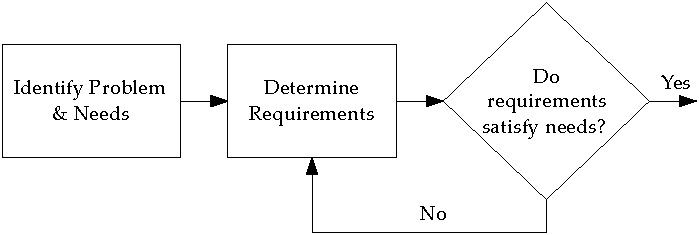
\includegraphics[width=3.8in,height=1.27in]{image1}
\caption{A prescriptive design process for problem
identification and requirements selection.}
\label{figure:prescriptiveDesign}
\end{figure}

A descriptive process that is widely applicable to design problems is
shown in Figure~\ref{figure:overviewDesignProcess}. 
In a perfect world, the process starts with the
identification of the problem, proceeds clockwise to research, followed
the requirements phase, and so on until the system or device is
delivered and goes into service (maintenance phase). This scenario is
unrealistic, ignoring the iterative nature of design where the design
team alternates between different phases as necessary. Consequently,
links are inserted that allow transitions between all the different
phases of the

\begin{figure}[h]
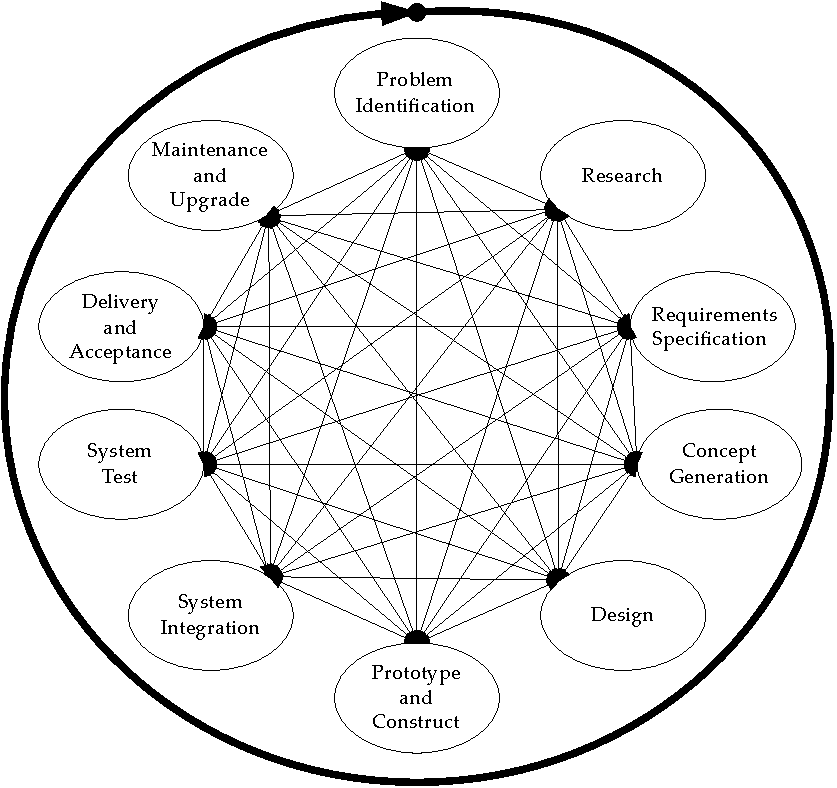
\includegraphics[width=5in,height=4.7in]{image2}
\caption{ A descriptive overview of the design process.}
\label{figure:overviewDesignProcess}
\end{figure}

design process. Of course, transitions between certain phases are
unreasonable or very costly. It is virtually impossible to move directly
from problem identification to system integration without developing a
design concept first. It is much more likely for engineers to alternate
between nearby phases in the process, such as problem identification,
research, requirements specification, and concept generation. This does
not mean that you can't move between phases that are not in close
proximity in the model. For instance, the customer's needs may change
while in the design phase, necessitating re-evaluation of the needs,
correction of the requirements specification, and system redesign---all
at a substantial cost in time and money. Studies have shown that the
cost required to correct errors or make changes increases exponentially
as the project lifetime increases, as presented in Figure~\ref{figure:costVsLife}.

\begin{figure}[h]
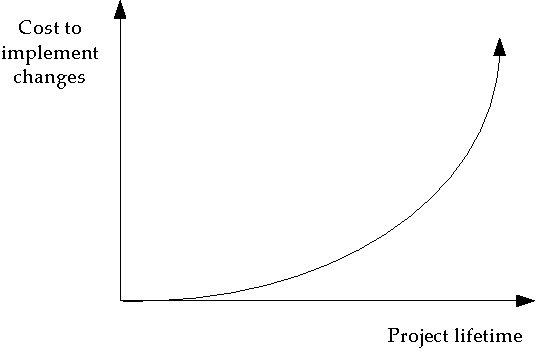
\includegraphics[width=3in,height=2in]{image3}
\caption{The cost to implement design changes increases exponentially with project lifetime.}
\label{figure:costVsLife}
\end{figure}

\subsection{Elements of the Design Process}

Nearly all the phases of the design process in Figure~\ref{figure:overviewDesignProcess} 
are covered in this book, with the exception of the maintenance phase. The objective of
the first phase, \emph{\textbf{problem identification}}, is to identify
the problem and customer needs. This occurs in a variety of ways, from
someone conceiving a new idea to a client coming to you with a problem
to solve. In either case, it is important to determine the true needs
for the product, device, or system (terms that are used interchangeably
throughout the book and often referred to as systems). Failure to
correctly identify the needs has negative ramifications for the entire
process, typically resulting in costly redesigns, or even worse,
abandonment of the project.

In the \emph{\textbf{research phase}} the design team conducts research
on the basic engineering and scientific principles, related
technologies, and existing solutions. The objective is to become experts
on the problem, save time and money by not re-inventing the wheel, and
be positioned to develop new and innovative solutions.

The \emph{\textbf{Requirements Specification}} articulates what the
system must do for it to be successful and to be accepted by the
customer. It is important to focus on what the system must do, as
opposed to how the solution will be implemented. This is challenging
since engineers tend to focus on solutions and propose implementations
early in the process. This is not surprising since engineering education
focuses on solving problems rather than specifying them. The
requirements are the mission statement that guides the entire project,
and if properly developed, provide flexibility for creativity and
innovation in developing solutions.

In \emph{\textbf{concept generation},} many possible solutions to the
problem are developed. The hallmark of design is that it is open-ended,
meaning that there are multiple solutions to the problem and the
objective is to develop the one that best meets the requirements and
satisfies the constraints. In this phase, wild creativity is encouraged,
but it is ultimately tempered with critical evaluation of the competing
alternatives.

In the \emph{\textbf{design phase},} the team iteratively develops a
technical solution, ultimately producing a detailed system design. Upon
its completion, all major systems and subsystems are identified and
described using an appropriate model that depends upon the particular
technology being employed.

In the \emph{\textbf{prototyping and construction phase},} different
elements of the system are constructed and tested. In rapid prototyping,
the objective is to model some aspect of the system, demonstrating
functionality to be employed in the final realization. Many prototypes
are discarded or modified as the system evolves---the idea is to
experiment, demonstrate proof-of-concept principles, and improve
understanding. Prototypes may be used anywhere in the process---you may
present the client with prototypes after the concept generation phase,
or they may be utilized in the design phase to test a design idea, or as
the final system is tested and developed.

During \emph{\textbf{system integration},} all of the subsystems are
brought together to produce a complete working system. This phase is
challenging and time-consuming since many different pieces of the design
must be interfaced, and the team must work closely to make it all work.
Care taken in the design phase to clearly communicate the functionality
and interfaces between subsystems aids in system integration. System
integration is closely tied to the \emph{\textbf{test phase}}, where the
overall system is tested to demonstrate that it meets the requirements.

Ultimately the system is \emph{delivered} to the customer where it is
likely that they will test it using a mutually agreed upon process.
Development does not necessarily end when the system goes into service,
as it will likely enter the \emph{\textbf{maintenance phase}} where it
is maintained, upgraded to add new functionality, or where design
problems are corrected. Following and understanding the design process
improves the probability of successful system development. The process
is flexible, and the designer needs to transition between different
phases in order to bring the system to realization. Design is an
iterative process---you may not fully understand everything necessary in
any given phase and have to revisit different steps as the system
evolves. That is not a license for not trying to develop the best design
you can on the first attempt---by all means do so---but realize that
flexibility and a willingness to change the design are necessary.

\subsection{Technology Specific Design Processes}

Different application domains have developed specialized processes for
technology-specific design. One such example is VLSI (Very Large Scale
Integration) design. A typical VLSI design process is shown in Figure~\ref{figure:VLSIdesign}
 {[}Wol02{]}. In this model the system specification is used to
develop the system architecture. The system architecture is composed of
the major functional units that constitute an integrated circuit. Each
functional unit is then designed at the gate logic level, which is
subsequently designed at the circuit (transistor) level, and finally the
circuit elements are laid out on the silicon chip. This is an excellent
demonstration of the divide-and-conquer approach to design, where a
complex system is broken down into lower levels of abstraction and each
of these is further broken down until the design objectives are met.

\begin{figure}[h]
 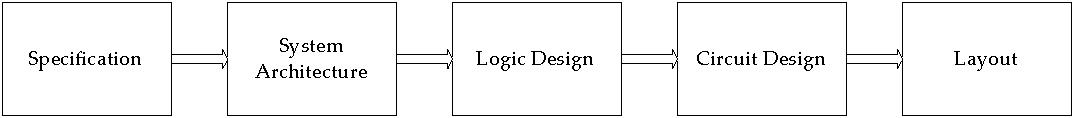
\includegraphics[width=5.5in,height=0.60417in]{image4}
\caption{A process for integrated circuit (VLSI) design {[}Wol02{]}.}
\label{figure:VLSIdesign}
\end{figure}

Next, consider the design process for embedded computer systems shown in
Figure~\ref{figure:embedded DesignProcess}. 
Embedded systems are combined hardware/software systems
embedded into a larger system to perform dedicated application specific
operations. Embedded systems are employed in automobiles, DVD players,
and digital cameras to name a few applications. Performance issues
dominate embedded applications, and the designer needs to partition
tasks between software and hardware to achieve optimum performance. This
design process is somewhat prescriptive with phases for requirements
gathering, specifications, and architectural design. The process
reflects the unique nature of embedded systems with separate software
and hardware design blocks, married together by the interface design.

\begin{figure}[h]
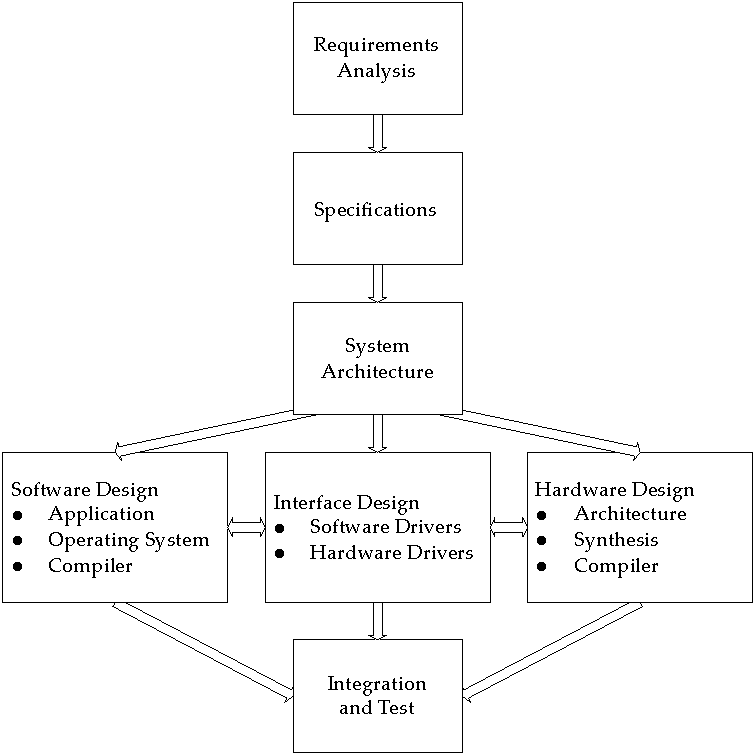
\includegraphics[width=3.8in,height=3.8in]{image5}
\caption{An embedded system design process {[}Ern97{]}.}
\label{figure:embedded DesignProcess}
\end{figure}

The field of software engineering is one in which the development of
different design process models is still under considerable flux today.
This is due to the complex nature of software and the failure of
computer scientists and engineers to effectively develop high-quality
software systems. There are many reasons why this is so. The sheer size
of software programs may easily exceed one million lines of code written
by many different software developers. One small mistake in those
millions of lines of code can cause the system to fail. Another
difficulty is in designing for upgrade and reuse of software. What if
the needs change after the millions of lines of code are developed and
one of the fundamental structures or objects needs to be upgraded?

The \emph{waterfall model} shown in Figure~\ref{figure:waterfallDesignProcess} 
is one of the first
proposed and most well-known software design processes. This is a
prescriptive model since the development proceeds linearly from the
first step where the user's needs are analyzed through the phases of
specification development, design, test, and maintenance. This works for
well-defined and moderately complex software applications, but fails as
complexity grows due to the inability to move between phases. A more
flexible and descriptive software design process is known as the
\emph{spiral model}, which is a cyclical process where phases are
revisited as necessary {[}Som01{]}. \emph{Extreme Programming} is a more
recent and controversial software development process, where relatively
small teams of software developers rapidly develop software following
some strict rules. Both the spiral model and Extreme Programming are
examined in more detail in the end of chapter problems.

\begin{figure}[h]
 
\includegraphics[width=4.6in,height=3.1in]{image6}
\caption{Waterfall software development process. In this
model, development proceeds linearly from requirements analysis, through
each subsequent phase, terminating with maintenance.}
\label{figure:waterfallDesignProcess}
\end{figure}

\section{The World-Class Engineer}\label{the-world-class-engineer}

The ability to effectively design is important for engineers, requiring
strong technical skills and an understanding of the design process. Yet,
this ability in itself is not enough to become an effective practicing
engineer. The Pennsylvania State University Leonhard Center for the
Advancement of Engineering Education, in consultation with a number of
industries, developed a description of what is referred to as a
``World-Class Engineer'' {[}Leo95{]}. Shown in Table~\ref{table:worldClassEngineer},
 the description identifies the characteristics of successful engineers, and
contains six major elements: 1) Aware of the World, 2) Solidly Grounded,
3) Technically Broad, 4) Effective in Group Operations, 5) Versatile,
and 6) Customer-Oriented. The description recognizes that engineers must
be effective in group operations, since the majority of projects are
carried out in teams. Not only that, many projects span multiple
technical disciplines and are executed in multifunctional organizations
that have diverse groups such as marketing, finance, human resources,
technical support, and service. It also recognizes that an engineer must
be versatile, innovative, understand ethical principles, and be
customer-oriented, important themes that are stressed throughout this
book.

\footnotesize
\begin{longtable}[c]{|m{14cm}|}
\caption{The World-Class Engineer (Copyright the Leonhard
Center for the Advancement of Engineering Education, The Pennsylvania
State University. Reprinted by permission.) 
\label{table:worldClassEngineer}}\\


\hline
\rowcolor{Gray}
\textbf{World Class Engineer} \\ \hline
\endfirsthead

\hline
\rowcolor{Gray}
{{\bfseries \tablename\ \thetable{} -- continued from previous page}} \\ \hline
\rowcolor{Gray}
\textbf{World Class Engineer} \\ \hline
\endhead
\endfoot

\hline

\begin{enumerate}
\itemsep0em 
\def\labelenumi{\Roman{enumi})}

\item Aware of the World 
\begin{itemize}
\itemsep0em 
\item  sensitive to cultural differences, environmental concerns, and ethical  principles
\item  alert to market opportunities (both high- and low-tech)
\item  cognizant of competitive talents, work ethic, and motivation
\end{itemize}

\item Solidly Grounded
\begin{itemize}
\itemsep0em 
\item  thoroughly trained in the fundamentals of a selected engineering
  discipline
\item  has a historical perspective and remains aware of advances in science
  that can impact engineering
\item  realizes that knowledge doubles at breakneck speed and is prepared to
  continue learning throughout a career
\end{itemize}

\item Technically Broad
\begin{itemize}
\itemsep0em 
\item  understands that real-life problems are multidisciplinary
\item  thinks broadly, seeing an issue in a rich context of various
  alternatives, probabilities, etc., rather than a narrow quest to find
  a single answer
\item  is conversant in several disciplines
\item  is trained in systems modeling and the identification of critical
  elements. Understands the need to design experiments to verify or
  extend analysis, as well as meet specification requirements
\item  is psychologically prepared to embrace any field necessary to solve
  the problem at hand
\end{itemize}

\item Effective in Group Operations
\begin{itemize}
\itemsep0em 
\item  cooperative in an organization of individuals working toward a common
  creative goal that is often multidisciplinary and multifunctional in
  nature
\item  effective in written and oral communication
\item   willing to seek and use expert advice
\item  cognizant of the value of time and the need to make efficient use of
  the time in all phases of an endeavor
\item   understanding and respectful of the many facets of business operation
  -\/- general management, marketing, finance, law, human resources,
  manufacturing, service, and especially quality
\end{itemize}

\item Versatile
\begin{itemize}
\itemsep0em 
\item  innovative in the development of products and services
\item  sees engineering as applicable to problem solving in general
\item  considers applying engineering beyond the typical employment focus of
  engineering graduates in the manufacturing industries, to the much
  broader economy (financial services, health care, transportation,
  etc.) where engineering skills could make a dramatic improvement in
  the productivity of those segments of the economy that employ 80
  percent of the U.S. population
\end{itemize}

\item Customer Oriented 
\begin{itemize}
\itemsep0em 
\item  realizes that finding and satisfying customers is the only guarantee
  of business success
\item  understands that products and services must excel in the test of
  cost-effectiveness in the global marketplace
\end{itemize}
\end{enumerate}
\\ \hline
\end{longtable}
\normalsize




\section{Book Overview}\label{book-overview}

Consider the digital camera, the cellular phone, and the space shuttle,
all complex systems that integrate a variety of technologies. A digital
camera is the synthesis of an embedded electronics system, optics, a
mechanical lens assembly, and the camera package itself. The embedded
electronics contain an imaging sensor, a digital display, digital
interface circuitry, flash memory storage, system control software, and
the user interface. The challenges of integrating the components of such
a system and having it record and transfer huge amounts of image data,
within an acceptable timeframe, are immense. Cellular phones are another
good example of a complex system that represents a technology that has
shrunk in size, but increased tremendously in functionality at the same
time. They encompass digital data communications, antenna design,
encryption for secure data transmission, a user interface display, and
Internet connectivity. At the other end of the spectrum are large-scale
space and military systems, such as the space shuttle. Despite the two
shuttle accidents, the safety and reliability requirements of the space
shuttle are incredibly high. Realizing such a system is accomplished by
a tremendous number of people from many disciplines working for
different organizations. All three of these technologies were developed
by large teams that encompass multiple disciplines. The processes and
practices employed in their development represent application of the
fundamentals that this book hopes to cover. While you won't be building
complete space shuttles by the end of this design course, you can expect
to apply design principles that allow you to design and integrate a
relatively complex system, maybe even a part of the space shuttle.


The intention is to teach the application of design principles to
computer and electrical engineers and to help prepare students for a
professional career. The majority of engineering education is devoted to
math, science, engineering science, and problem-solving. They are
important topics required to enter this highly technical field. However,
it is clear that there are other aspects beyond this that are equally
important for success, including an understanding of system design,
innovation, ethical principles, teamwork, and strong communication
skills.

The book is divided into three parts: I--Design Process, II--Design
Tools, and III--Professional Skills. This is shown in Figure~\ref{table:bookPhilosophy}
 as three separate, but related components that play a key role in achieving
Project Excellence---the ability to complete a project, in an ethical
manner that meets the customer's need, satisfies the constraints, and is
clearly communicated to all involved. The chapters are decoupled as much
as possible so that the reader can move between chapters as necessary.
In Part I, the emphasis is on understanding and gaining experience in
the different phases of the design process. The reader is guided through
the steps of project identification, research, specification
development, creative concept generation, and critical evaluation of
competing solutions. Part II addresses topics that are often employed in
design, including functional decomposition, description of system
behavior, reliability, and testing. Part III addresses professional
skills, including teamwork principles, project planning, ethics in
design and the profession, and oral communication skills.

\begin{figure}[h]
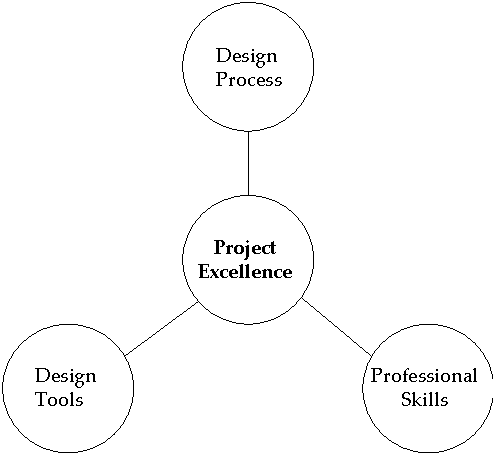
\includegraphics[width=2.875in,height=2.625in]{image7}
\caption{The guiding philosophy of this book. In order to
achieve success in executing engineering and design projects, it takes
an understanding of the design process, strong technical design tools,
and professional skills.}
\label{table:bookPhilosophy}
\end{figure}


Here are a few thoughts to conclude the chapter and get started on the
path to great designs. You are embarking on what will likely be a fun,
challenging, sometimes frustrating, and ultimately rewarding journey.
The systems that engineers work with continue to become increasingly
complex and multi-disciplinary in nature. The example problems presented
in this book come from the fields of analog electronics, digital
electronics, electrical systems theory, and software systems. These four
areas comprise a significant problem-domain common to the education of
most electrical and computer engineers. Finally, consider the quote
below by Robert Hayes on the importance of design.

Fifteen years ago, companies competed on price. Today it's quality.
Tomorrow it's design.---Robert H. Hayes, Harvard Business School, 1991.

What is this saying? Well, it is clear that the world continues to move
to a more knowledge-based society, where individuals and companies
compete on the strength of their intellectual capital and ability to
produce new and innovative products. That is what design is all about.
It is not saying that price and quality are unimportant, they certainly
are; in fact quality and reliability in design are part of this book. It
is that quality and price are a given, and successful products will be
distinguished by their design characteristics. The implication is that
design will play a larger role in the development and success of
products. The future Hayes predicted is now. Design is what
distinguishes between products that are seen as commodities and those
that are truly unique and profitable.

\section{Summary and Further
Reading}\label{summary-and-further-reading}

Engineering design is an iterative process in which the design team
employs creativity and technical knowledge to develop a solution that
best meets the end-users' needs within the constraints applied to the
problem. There is no single design process that can be applied to all
situations and technologies, but there are many common elements shared,
regardless of the technology under consideration. In order to
successfully bring designs to fruition, it takes a combination of design
tools, professional skills, and a clear understanding of the process
needed to complete designs. The objective of this book is to develop
your proficiency in these areas so that you may become an effective
engineer and achieve excellence in design projects.

\underline{Engineering Design Methods} by Nigel Cross {[}Cro00{]} presents the
differences between descriptive and prescriptive design processes, and
covers a wide array of processes in more detail. It also discusses the
cognitive characteristics of effective designers. There are many good
books on software engineering process development methods. \underline{Software
Engineering} by Ian Sommerville {[}Som01{]} discusses the different
software design process models, such as the waterfall and spiral models.
This is also true of many modern software engineering texts. The
original reference to the waterfall model is by Royce {[}Roy70{]}.
\underline{The Art of Innovation} by Michael Kelley {[}Kel01{]} describes the
activities of well-known design company IDEO and is a highly readable
description of their design practices. The ABC \emph{Nightline} news
program also produced an interesting segment on IDEO {[}ABC01{]} that
can be purchased at the ABC website. \underline{The Circle of Innovation} by
Tom Peters {[}Pet97{]} is another popular book that provides his
perspective on current trends in business and the importance of design.
